\documentclass[../practica_03.tex]{subfiles}

\begin{document}

    \begin{enumerate}
        \item $\theta(t) = (\sin(t), \cos(t))$

            $\theta: \real \rightarrow (x,y) \in \real^2 : \abs*{x} \leq 1 \wedge \abs*{y} \leq 1$

            \begin{itemize}
                \item $ \sin(t) $ sabemos que es continua en todos los $\real$
                \item $ \cos(t) $ sabemos que es continua en todos los $\real$
                \item $ \sin(t) + \cos(t) $ por algebra de limites es contina en todos los $\real$
            \end{itemize}

            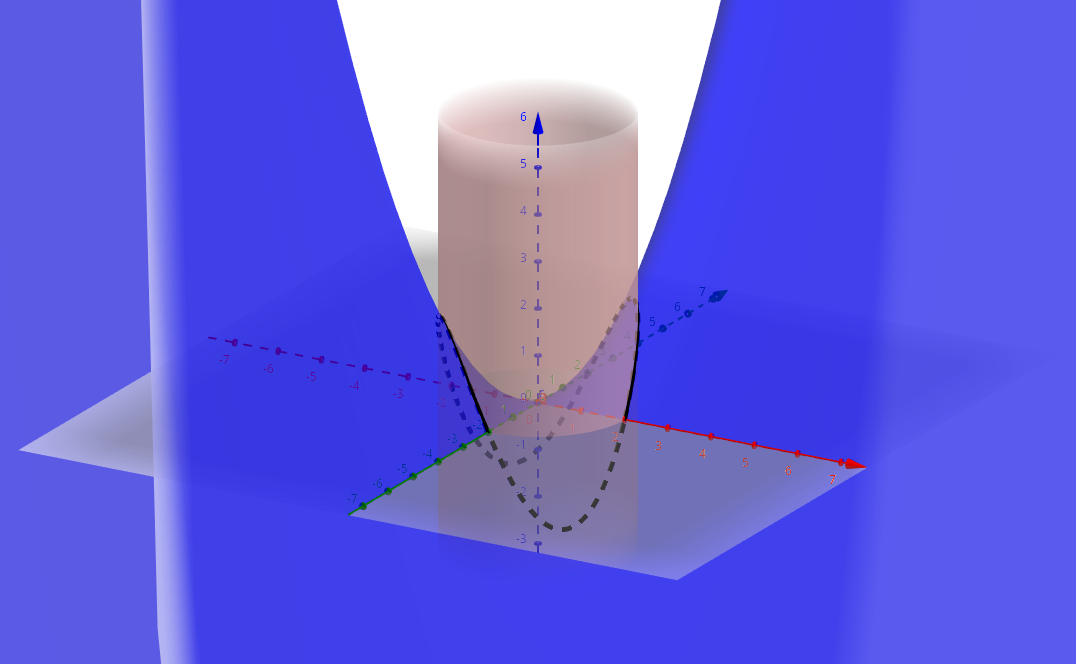
\includegraphics[scale=0.8]{ej01/resources/1a.png} $ $

        \item $\theta(t) = (\frac{\sin(t)}{t}, \ln(t^2-t), t^2)$

            \begin{itemize}
                \item $f(x) = \frac{\sin(t)}{t}$

                    $f: \real - {0} \rightarrow \real$

                    \begin{itemize}
                        \item $ \sin(t) $ es continua
                        \item $ t $ es continua
                        \item $ \frac{\sin(t)}{t} $ es continua en todos los puntos menos t = 0
                    \end{itemize}

                \item $g(x) = \ln(t^2-t)$

                    \begin{itemize}
                        \item $ t^2 -t $ es continua
                        \item $ \ln(t^2-t) $ es continua $\Leftrightarrow t^2 - t > 0$
                            $ t^2 - t > 0 \Leftrightarrow $
                            $ t^2 > t \stackrel{por\ f\ t \neq 0}{\Leftrightarrow} $
                            $ \abs*{t} > \sqrt{t} \equiv$
                            $ 0 < t < 1$
                    \end{itemize}

                    $g: \real - (0,1) \rightarrow \real $
                    
                \item $h(x) = t^2$

                    $h: \real \rightarrow \real $

                    $t^2$ es continua en todo $\real$

            \end{itemize}

            $\theta(t): \real - (0,1) \rightarrow \real^3$

            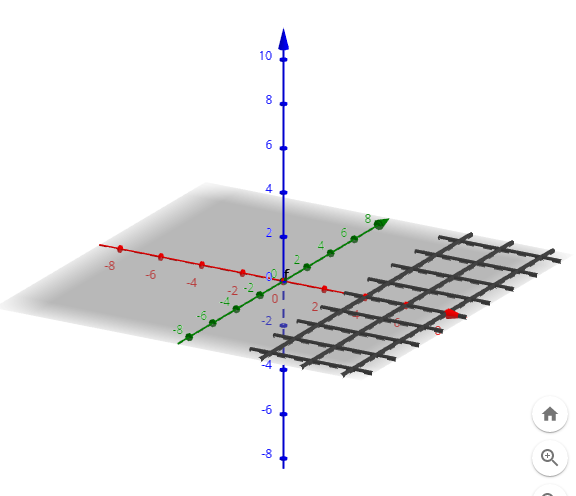
\includegraphics[scale=0.2]{ej01/resources/1b.png} $ $

        \item $\theta(t) = (\theta_1(t), \theta_2(t))$
            \begin{itemize}
                \item $\theta_1(t) = \sqrt{t}$
                \item $\theta_2(t) = \left\{
                        \begin{array}{ll}
                            \frac{\sin(t)}{t}\ si\ t \neq 0\\
                            1                \ si\ t = 0
                        \end{array}
                    \right.$
            \end{itemize}

            \begin{itemize}
                \item $\theta_1(t) = \sqrt{t}$
                
                    $\theta_1(t) : \real_{\geq 0} \rightarrow \real_{\geq 0}$

                    $\sqrt{t}$ Es continua en todo su dominio

                \item $\theta_2(t) = \left\{
                        \begin{array}{ll}
                            \frac{\sin(t)}{t}\ si\ t \neq 0\\
                            1                \ si\ t = 0
                        \end{array}
                    \right.$

                    $\theta_2(t): \real \rightarrow [1,-1]$

                    \begin{itemize}
                        \item $\frac{\sin(t)}{t}$ es continua en todos los puntos menos en $t=0$
                        \item $\theta_2(t) es continua \Leftrightarrow$
                        
                            $ \lim_{x\to0} \theta_2(t) = \theta_2(0) \Leftrightarrow$ 

                            $ \lim_{x\to0} \theta_2(t) = 1$ 

                            $ \lim_{x\to0} \frac{\sin(t)}{t} \stackrel{L'H}{\equiv}$ 

                            $ \lim_{x\to0} \frac{\cos(t)}{1} = 1$ 
                    \end{itemize}

                    $\Rightarrow \theta_2(t)$ es continua en todo su dominio $\blacksquare$

            \end{itemize}

            $\theta: \real_{\geq 0} \rightarrow \real^2 $

            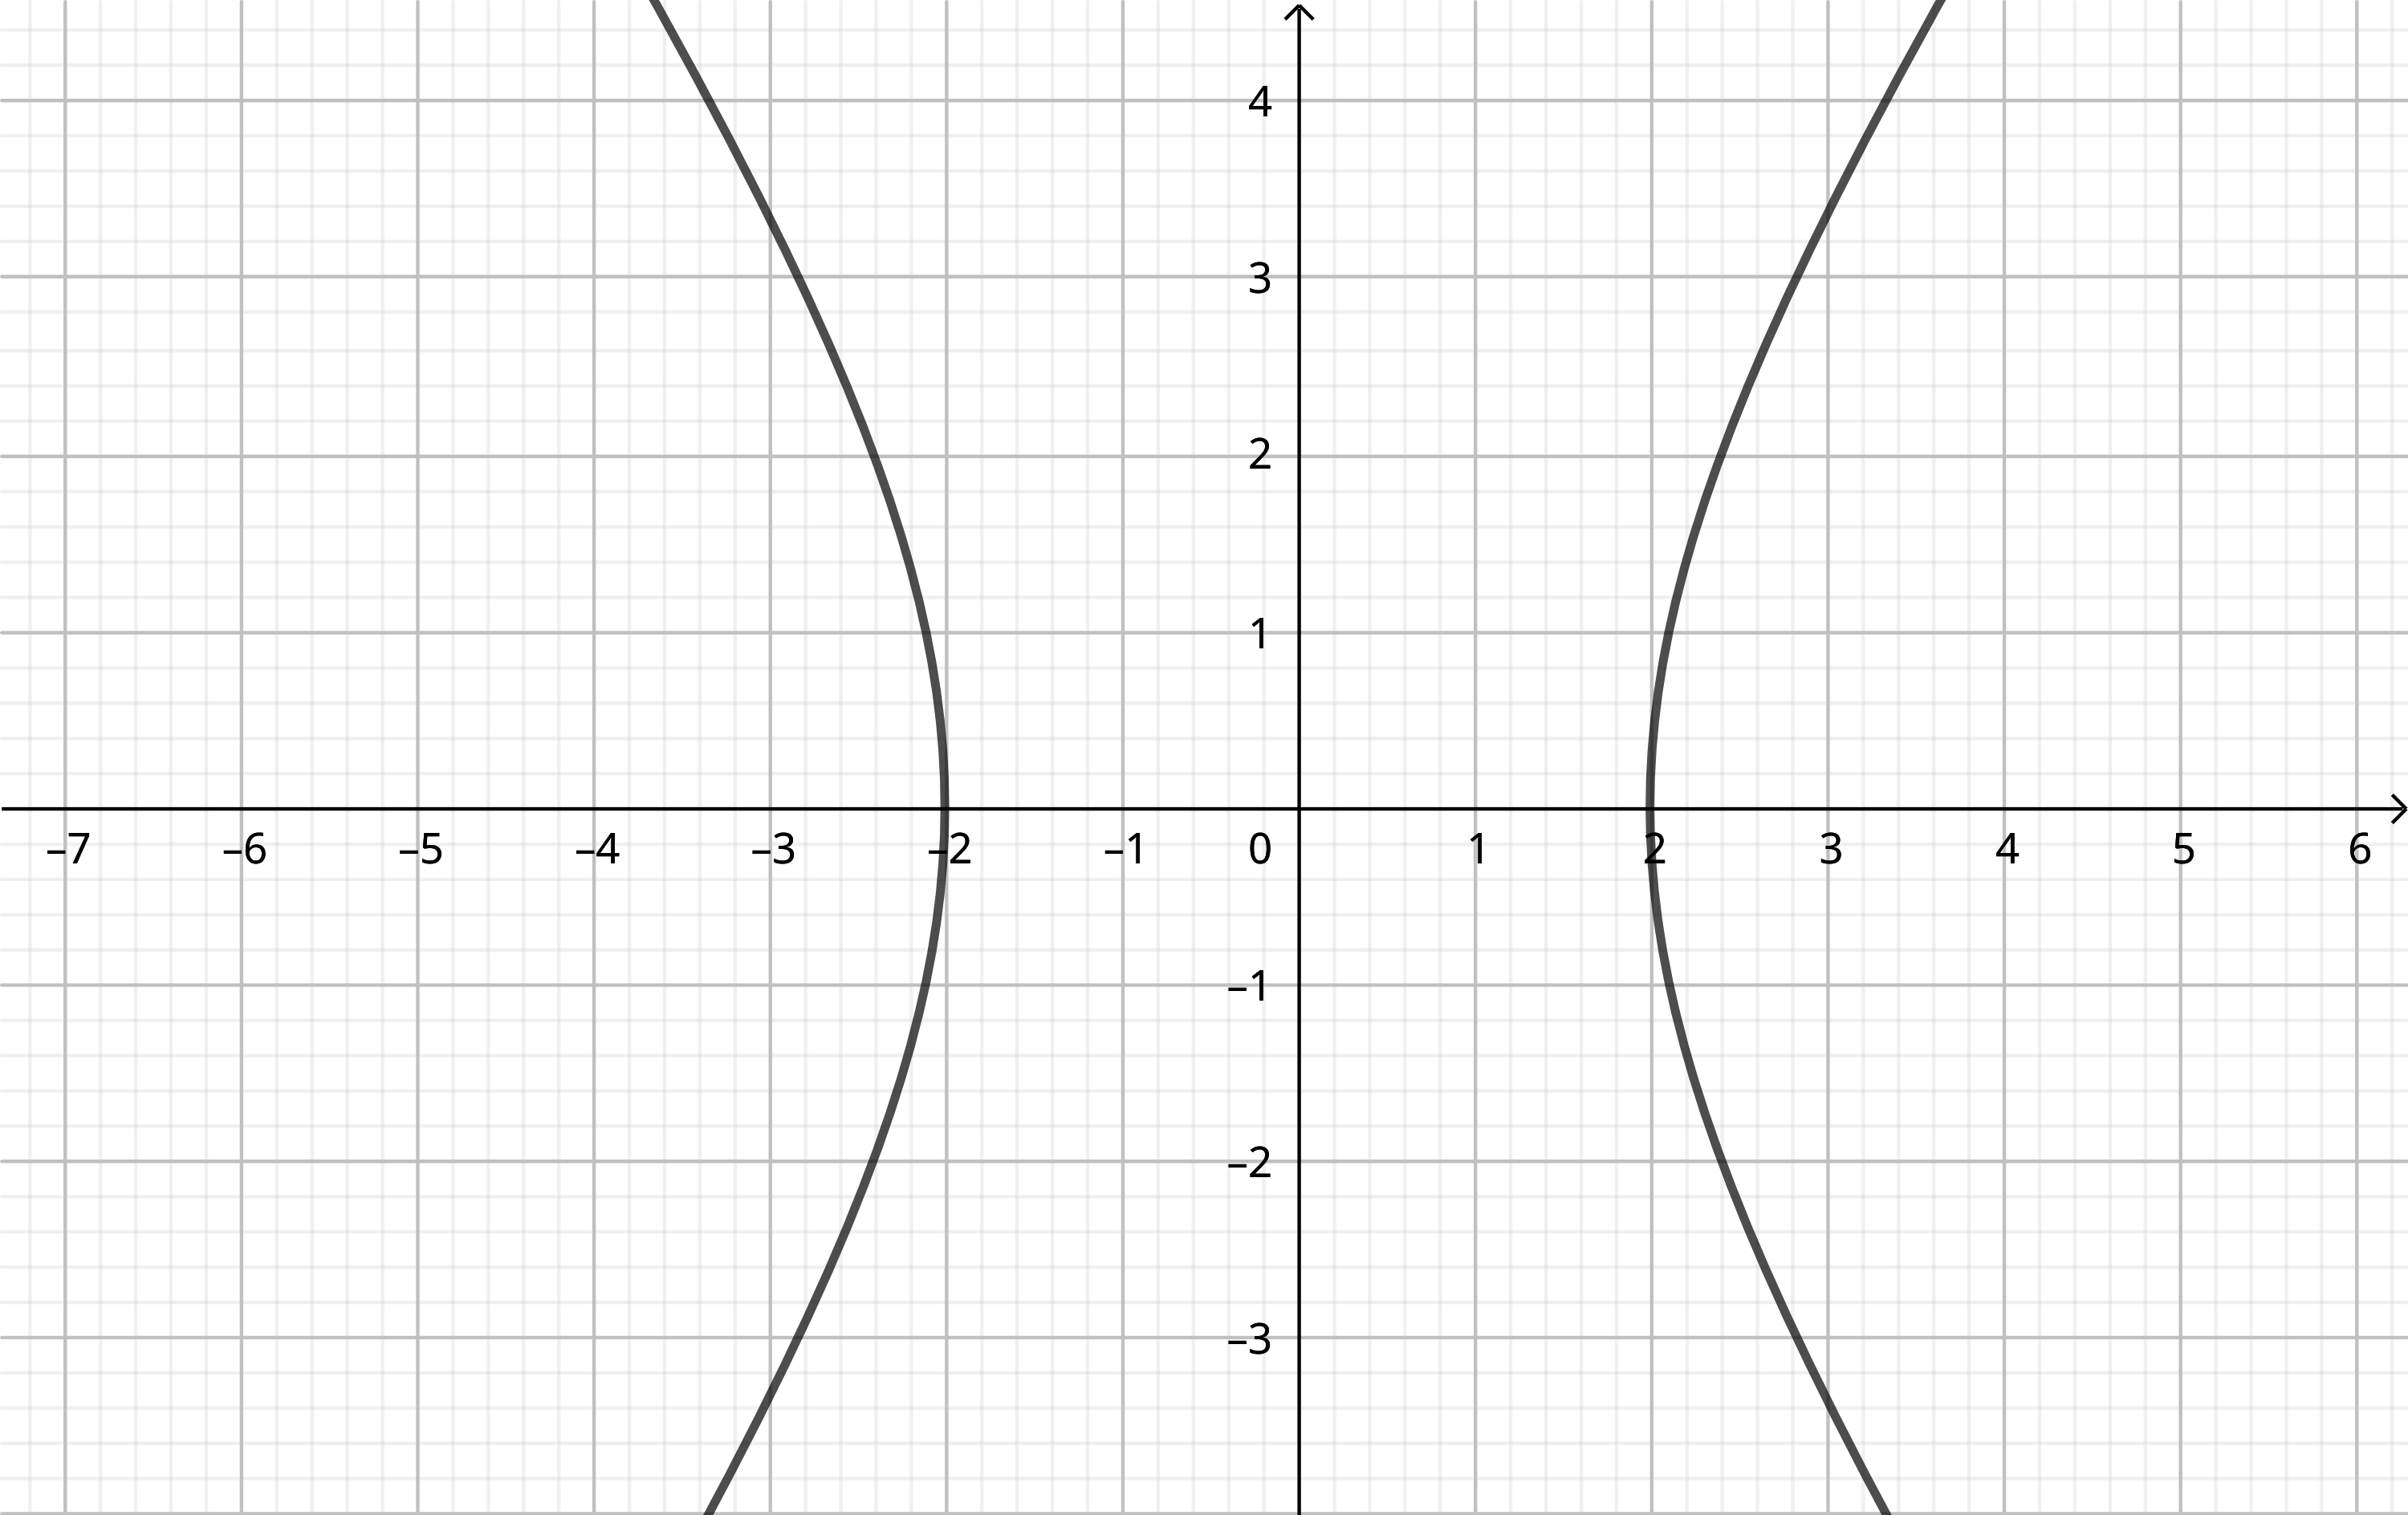
\includegraphics[scale=0.8]{ej01/resources/1c.png} $ $

    \end{enumerate}

\end{document} 
